\documentclass{article}
\usepackage[T1]{fontenc}
\usepackage{amssymb}
\usepackage{hyperref}
\usepackage{physics}
\usepackage{comment}
\usepackage{float}
\usepackage{graphicx}
\graphicspath{ {../FinalData/}{../EarlyData/}}

\usepackage{amsmath}
\usepackage[margin=2.5cm]{geometry}

\usepackage{nomencl}
\makenomenclature

\hypersetup{
    colorlinks,
    citecolor=black,
    filecolor=black,
    linkcolor=black,
    urlcolor=black
}

\title{Drag coefficient as a function of Mach number for PrawieR5 rocket}
\author{Manfred Gawlas}
\date{03.03.2024}


\begin{document}
\maketitle

\begin{comment}
	This documents shows resoults of flow simulations preformed in Solidworks on PrawieR5 rocket model. From those resoults graphs of drag coefficient as 		function of Mach number are then later analysed and compared to other in literature. Document also shows meshes and information about simulations.
\end{comment}

\begin{abstract}
	This paper presents the results of flow simulations conducted in Solidworks for the PrawieR5 rocket model. The ensuing drag coefficient graphs, as a 			function of Mach number, are analyzed and compared with Moder exterior ballistics. Additionally, the document discusses the utilized meshes and 				presents futher information about few choosen simulations.
\end{abstract}

\nomenclature{\(C_d\)}{Drag coefficient}
\nomenclature{\(A\)}{Area of cross-section of rocket}
\nomenclature{\(v\)}{Relative velocity}
\nomenclature{\(M\)}{Mach number}
\nomenclature{\(\rho\)}{Density of Air}
\nomenclature{\(k\)}{Specific heat ratio}
\printnomenclature

\section{Problem of drag coefficient}
\begin{comment}
This simple study will not take into account the complex nature of aerodynamic drag and will simplify drag effect to a simple equation for geometric and 		friction forces. This is to introduce a single drag coefficient, which we will treat as a function of Mach number. In that regard this study will strive to give 			similar plot to the ones for projectiles in Modern Exterior Ballistics.
\end{comment}
This basic study does not take into account the complex nature of aerodynamic drag and simplifies drag effect to a one minimal equation for geometric 			and friction forces. The aim is to establish a singular drag coefficient, treated as a function of Mach number. This study seeks to produce plot resembling 			those found in Modern Exterior Ballistics for projectiles.

\subsection{Basic physics used in study}
This study will focus on one drag coefficient, which in this case will be determined with usage of the equation from Modern exterior ballistics\cite{MEB}, which is showed bellow.
\begin{equation}
F_d = C_d \cdot A \cdot \frac{\rho_{air}v^2}{2}
\end{equation}

\subsection{CFD model}
\begin{comment}
Like mentioned already, simulations were conducted in Solidworks Flow Simulations. Initial conditions were: 

Mach number was changed by changes. Depending on simulation, different meshes were used for low mach and high mach parametric studies. For the high mach parametric study(>=3mach flow) high mach flow option was used in Solidworks settings. 
\end{comment}
As mentioned previously, simulations were conducted using Solidworks Flow Simulations. Initial conditions of simulation:

\begin{figure}[H]
\centering
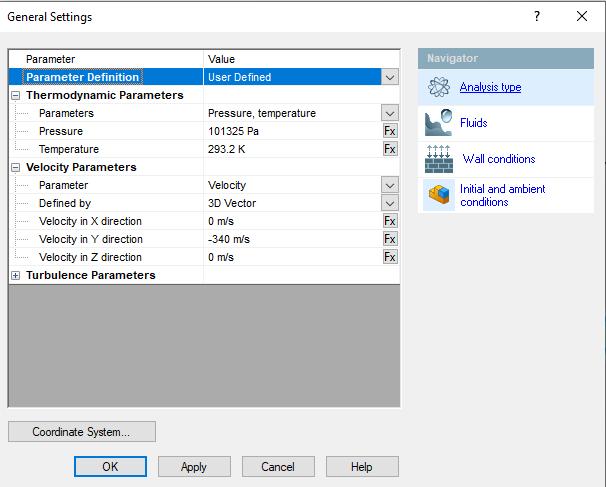
\includegraphics{GENERALSETTING}
\caption{Initial conditions}
\label{fig:GENERALSETTING}
\end{figure}

Mach number change was dependant only on changes in velocity. Depending on the simulation, different meshes were applied for parametric studies at low and high Mach numbers. For high Mach parametric studies (Mach number greater than or equal to 3), the high Mach flow option in Solidworks settings was utilized.


\section{Initial studies}
\subsection{General observations}
Initial studies dealt with problem of choosing correct settings for simulations. Most important highlight of this part is that high mach number setting should be choosen only when flow speed is close to Mach 3 or greater. Other big highlight is that Solidworks gives a warning for supersonic flows, but there is nothing we can do about it. It just gives a warning, there seem to be no setting that would get rid of it.\\\\
In this sections images of velocity and pressure graphs for high mach setting on will be shown, which later can be compared to high mach setting off, which is correct setting for those speeds. Bellow, reader can find mesh visualization for following simulations.
\begin{figure}[H]
\centering
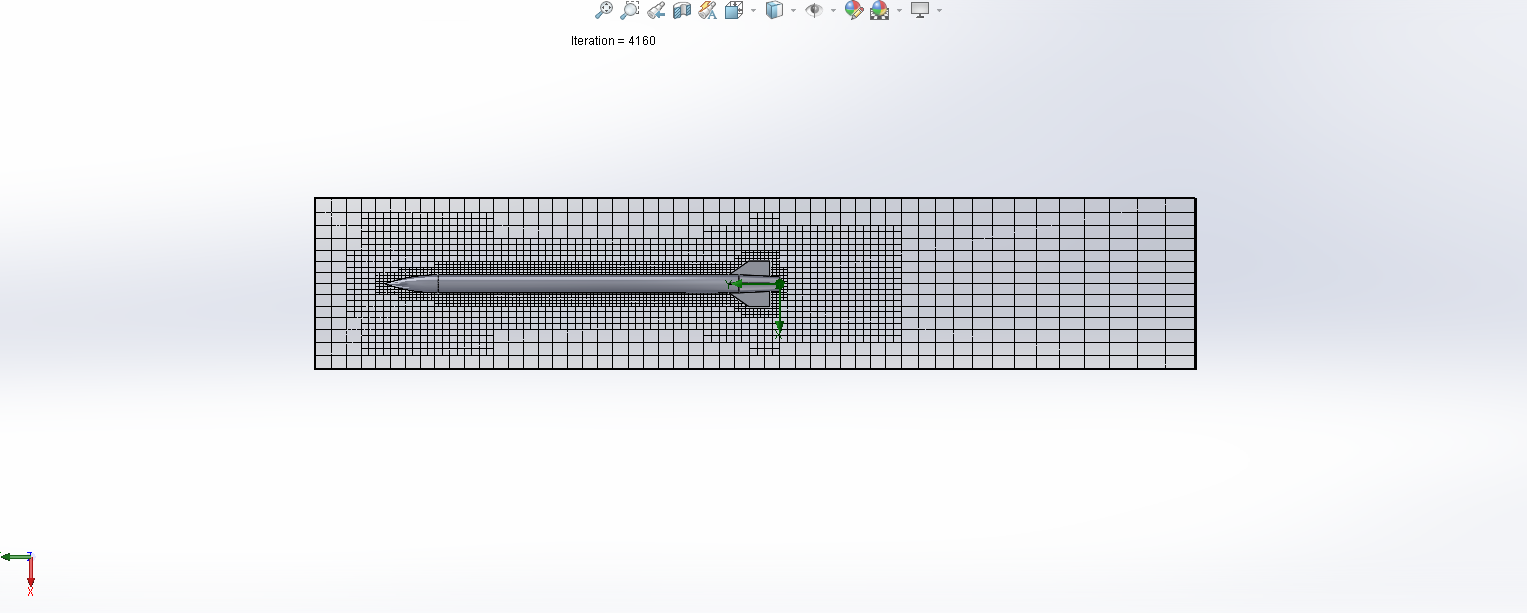
\includegraphics[width=\textwidth]{Mach1Mesh}
\caption{Mesh visualisation}
\label{fig:Mach1Mesh}
\end{figure}
\subsection{High mach setting on for Mach 0.8}
\begin{figure}[H]
\centering
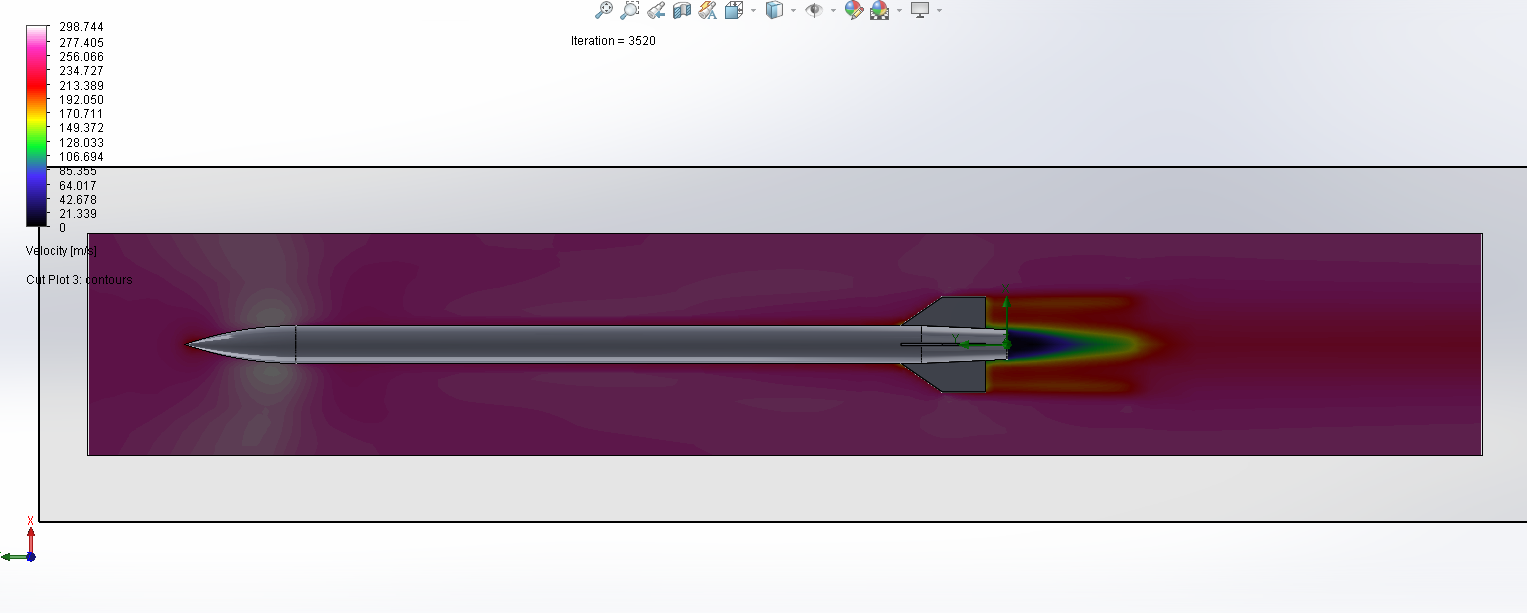
\includegraphics[width=\textwidth]{Mach08Speed}
\caption{Mach 0.8 velocity graph}
\label{fig:Mach08Speed}
\end{figure}

\begin{figure}[H]
\centering
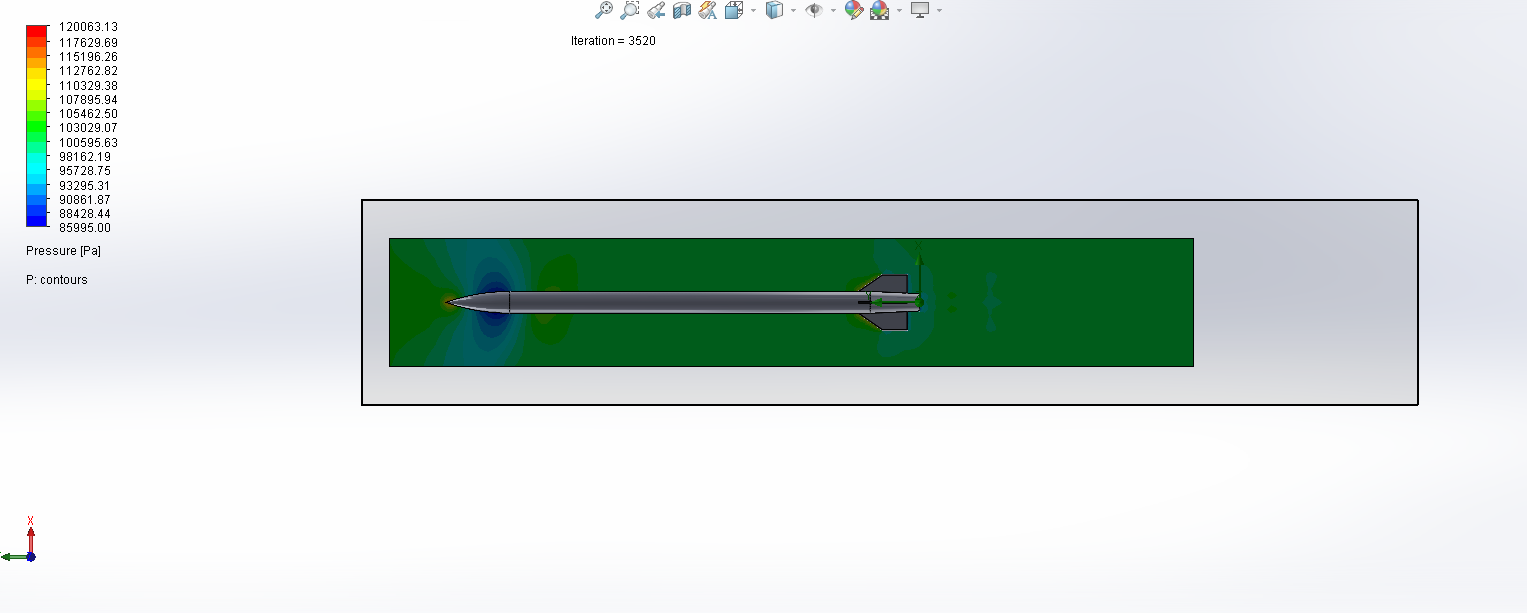
\includegraphics[width=\textwidth]{Mach08Pressure}
\caption{Mach 0.8 pressure graph}
\label{fig:Mach08Pressure}
\end{figure}

\subsection{High mach setting on for Mach 1}
\begin{figure}[H]
\centering
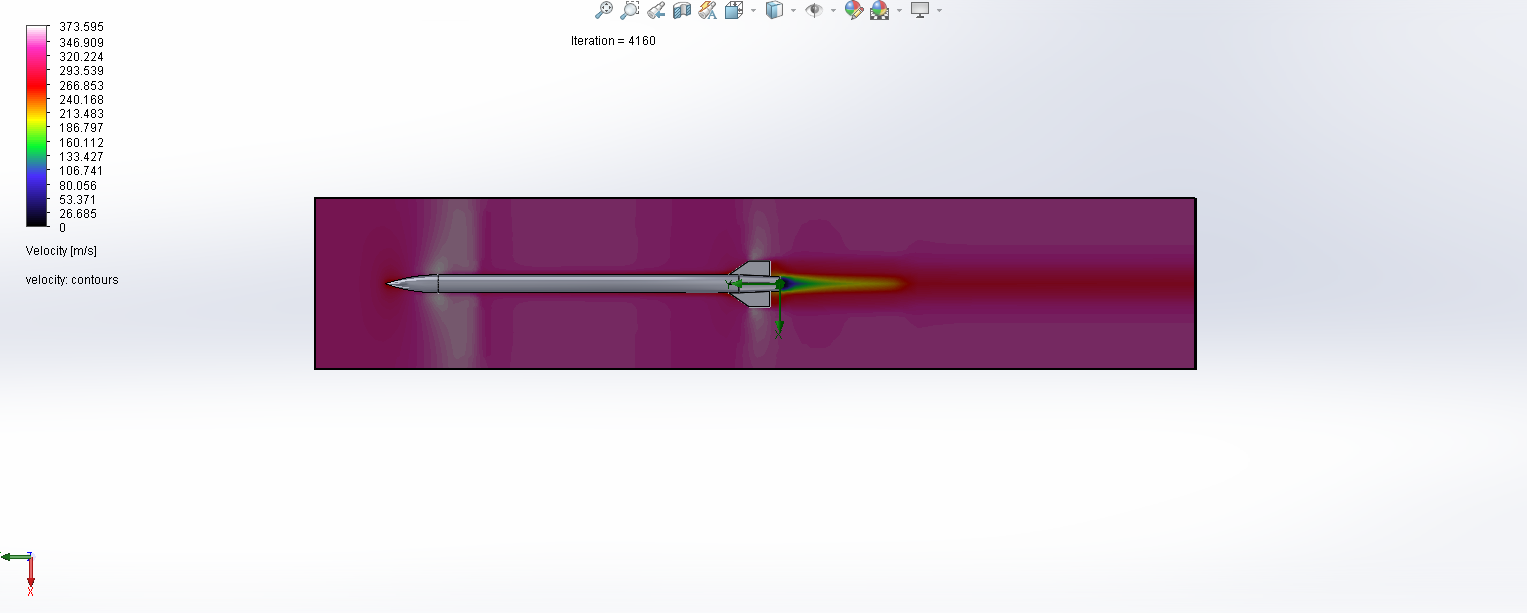
\includegraphics[width=\textwidth]{Mach1Speed}
\caption{Mach 1 velocity graph}
\label{fig:Mach1Speed}
\end{figure}

\begin{figure}[H]
\centering
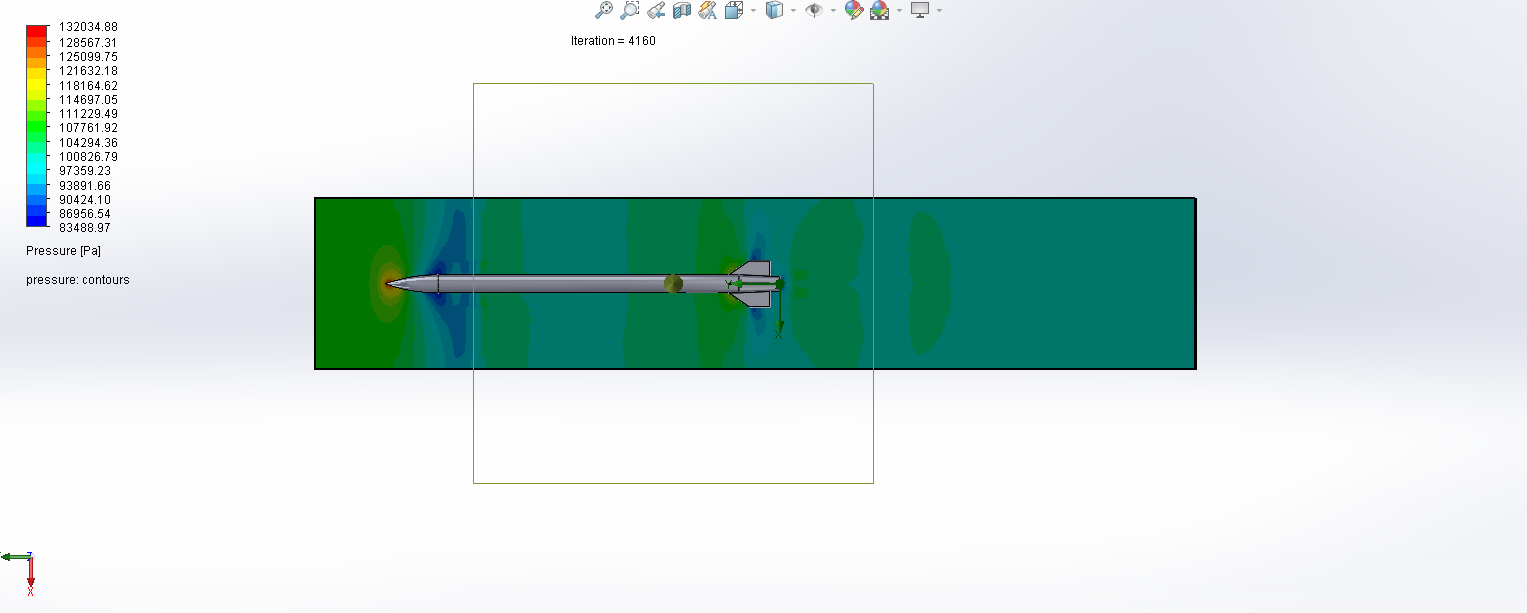
\includegraphics[width=\textwidth]{Mach1Pressure}
\caption{Mach 1 pressure graph}
\label{fig:Mach1Pressure}
\end{figure}


\section{Parametric study for low mach}
\subsection{General information}
After testing phase final simulations were conducted. For Range of 0 - 2.5 Mach high mach setting was turned off and new mesh was prepared. Since computational power avaible for the study was relativly small, parametric study was conducted for values of 0.2 - 1.6 Mach with step 0.1 Mach. Two additional points for study were used which were 2.0 and 2.5 Mach.

\subsection{Mesh settings}

\begin{figure}[H]
\centering
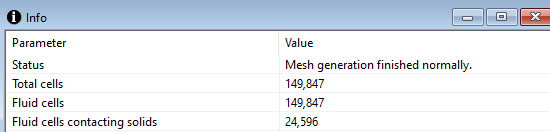
\includegraphics[width=\textwidth]{MESHCELLS}
\caption{Number of cells}
\label{fig:MESHCELLS}
\end{figure}

\begin{figure}[H]
\centering
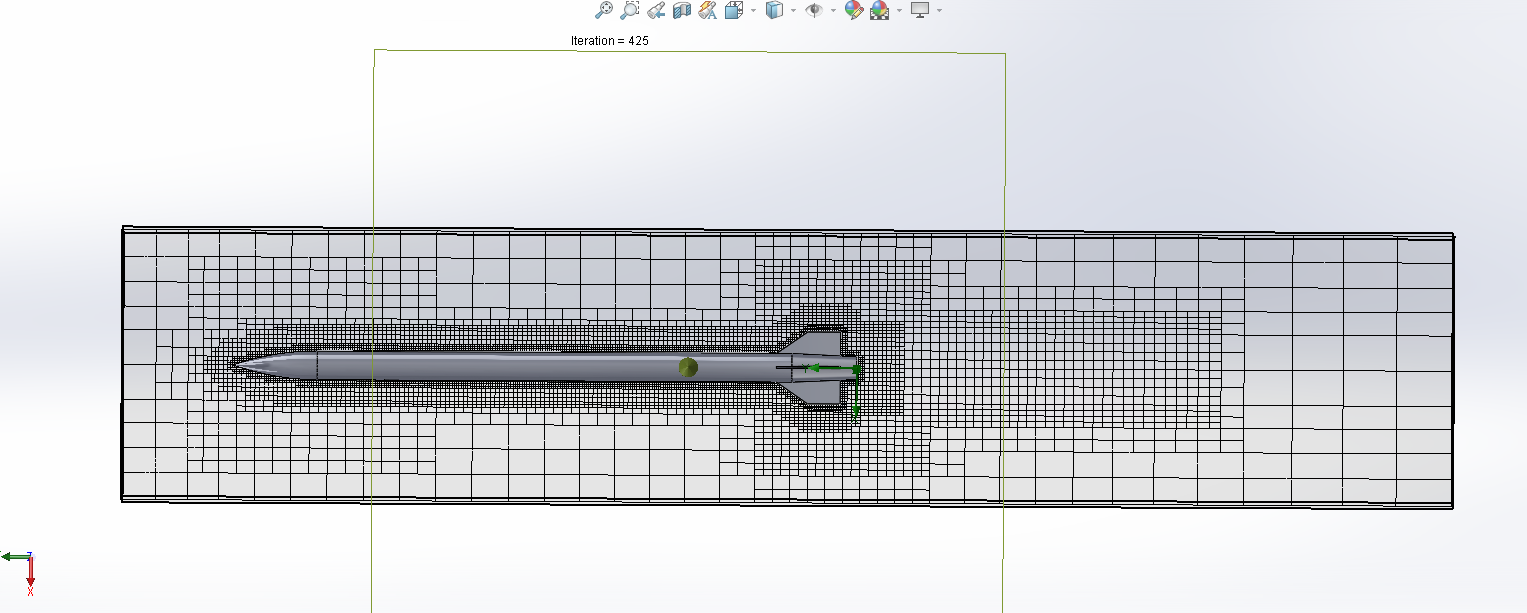
\includegraphics[width=\textwidth]{FinalMESH}
\caption{Mesh visualisation}
\label{fig:FinalMESH}
\end{figure}

\subsection{Mach 1 flow}
\begin{figure}[H]
\centering
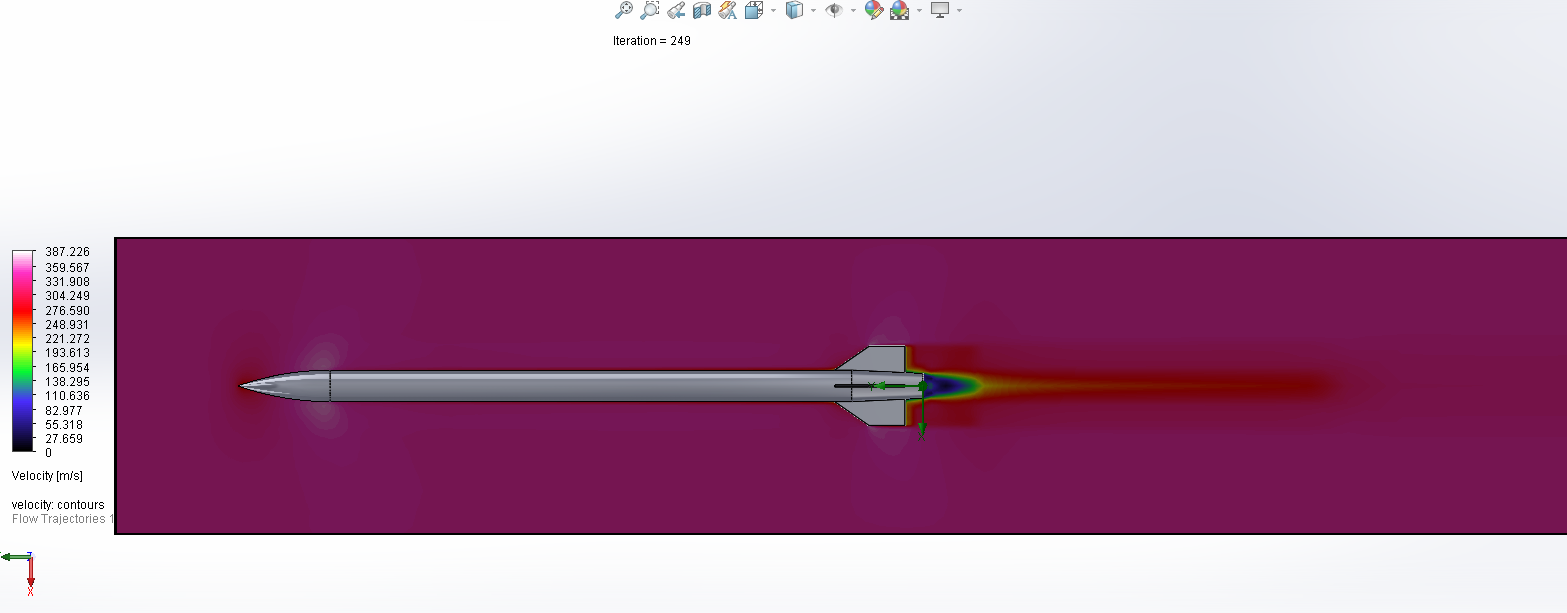
\includegraphics[width=\textwidth]{Final10Speed}
\caption{Mach 1 velocity graph}
\label{fig:Final10Speed}
\end{figure}

\begin{figure}[H]
\centering
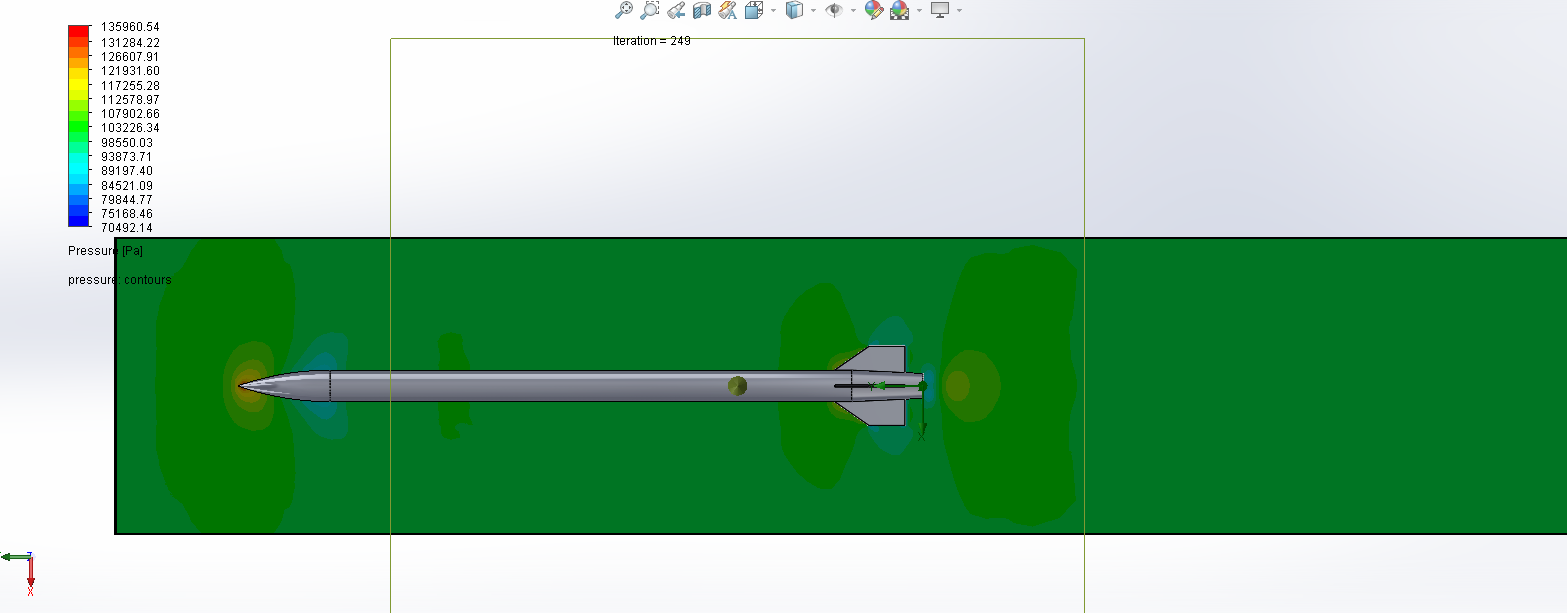
\includegraphics[width=\textwidth]{Final10Pressure}
\caption{Mach 1 pressure graph}
\label{fig:Final10Pressure}
\end{figure}

\subsection{Mach 1.6 flow}
\begin{figure}[H]
\centering
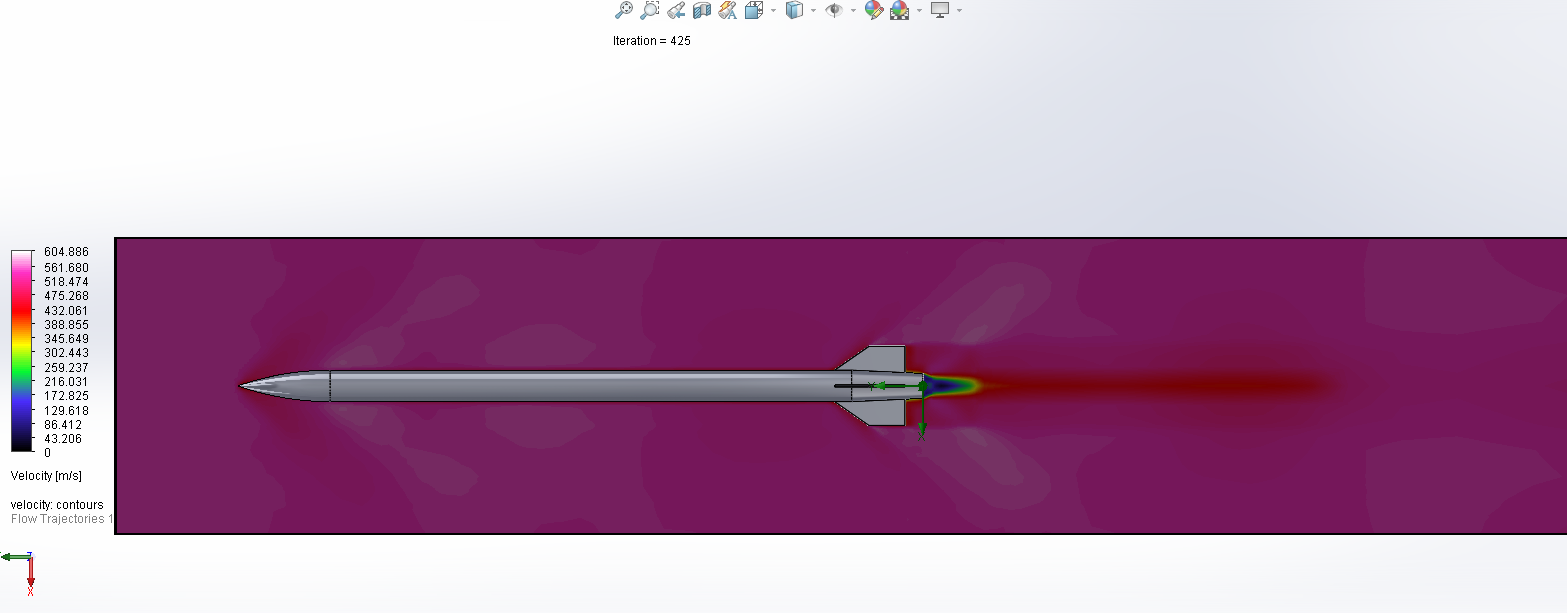
\includegraphics[width=\textwidth]{Final16Speed}
\caption{Mach 1.6 velocity graph}
\label{fig:Final16Speed}
\end{figure}

\begin{figure}[H]
\centering
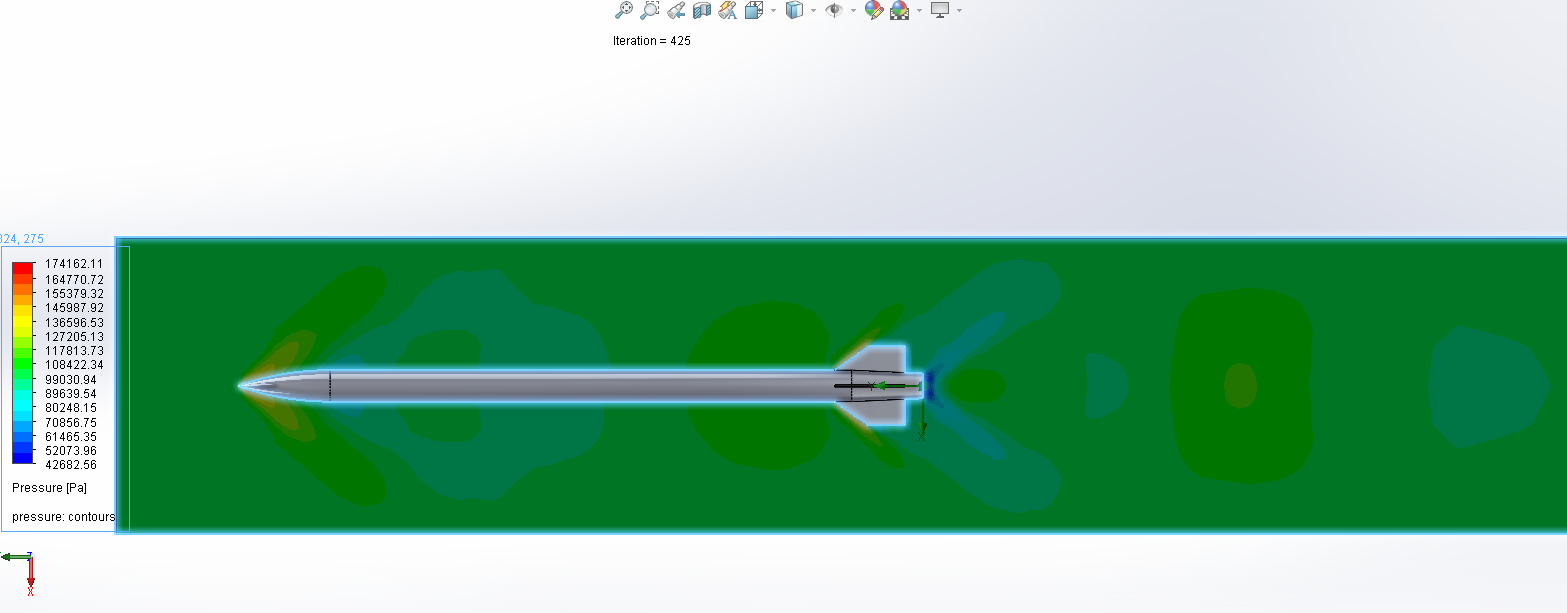
\includegraphics[width=\textwidth]{Final16Pressure}
\caption{Mach 1.6 pressure graph}
\label{fig:Final16Pressure}
\end{figure}

\subsection{Mach 2.5 flow}
\begin{figure}[H]
\centering
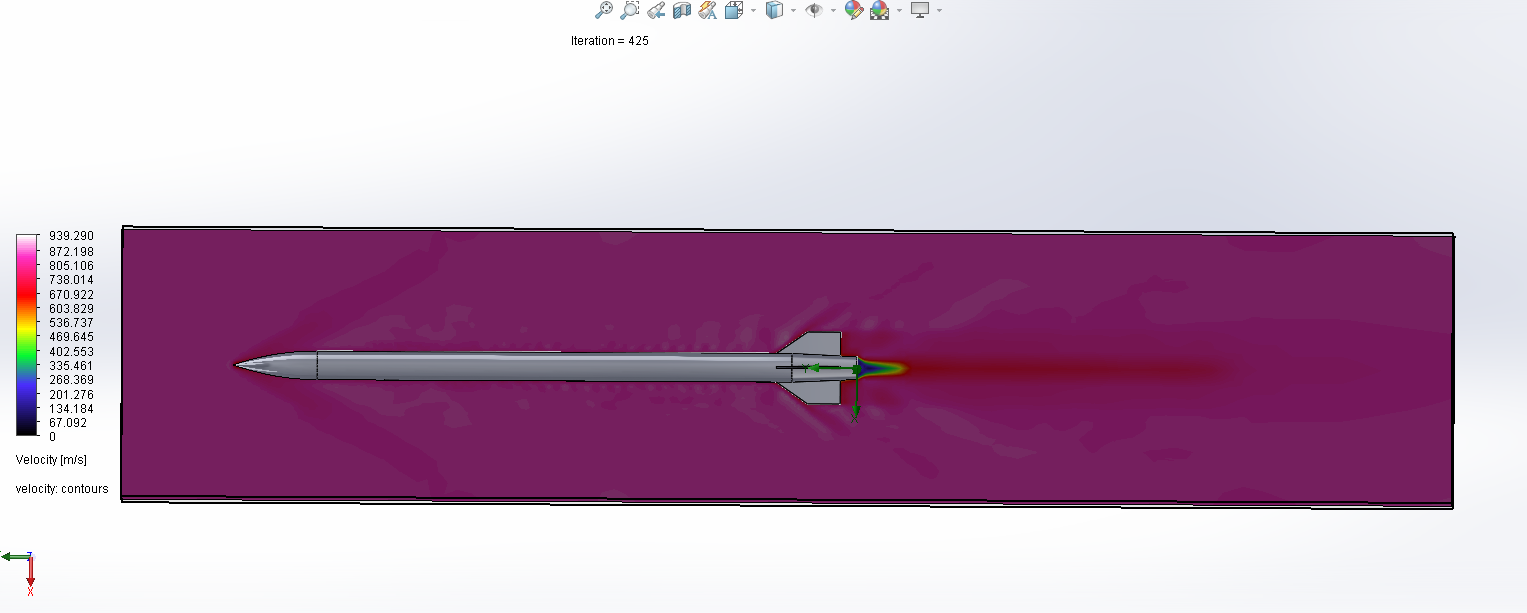
\includegraphics[width=\textwidth]{Final25Speed}
\caption{Mach 2.5 velocity graph}
\label{fig:Final25Speed}
\end{figure}

\begin{figure}[H]
\centering
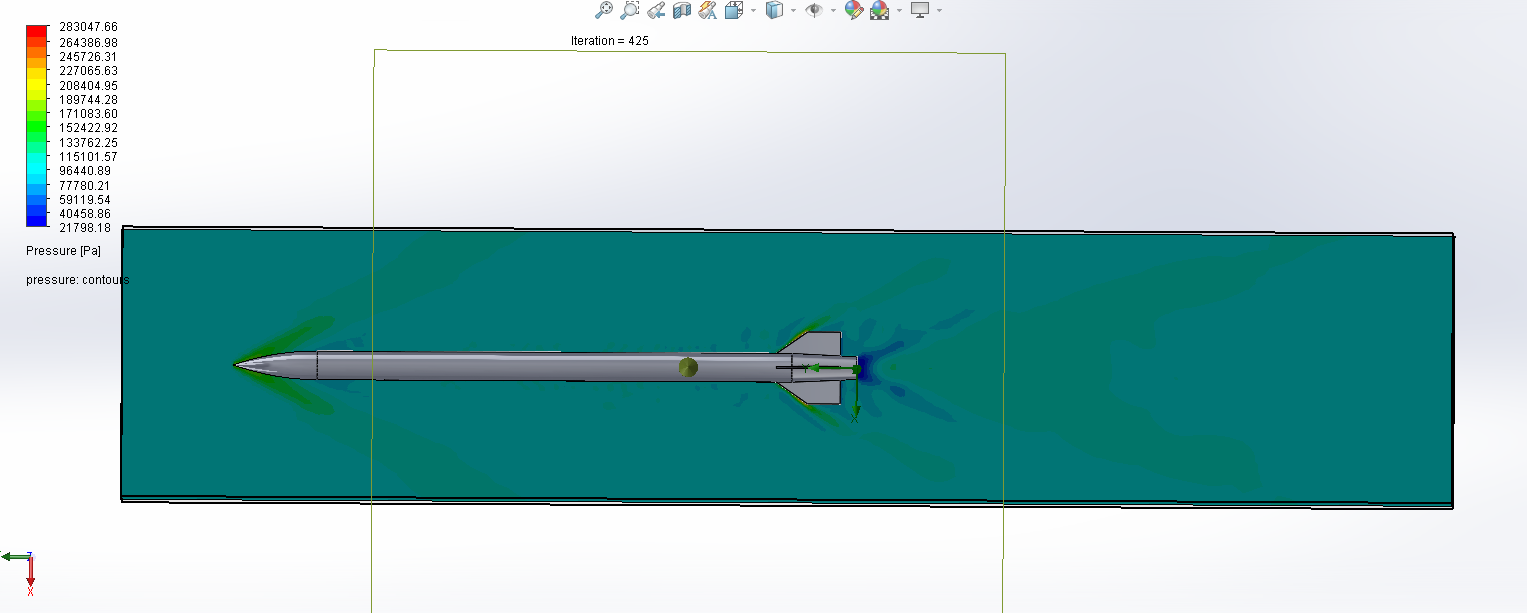
\includegraphics[width=\textwidth]{Final25Pressure}
\caption{Mach 2.5 pressure graph}
\label{fig:Final25Pressure}
\end{figure}

\section{Parametric study for high mach}
This parametric study was once again conducted for limited set of Mach values, starting from 3.0 to 5.0 with step equal to 0.5 Mach. The high mach setting was on for this series of simulations.

\subsection{Mach 5 flow}

\section{Results}
\subsection{General information}
As a result of the parametric studies, tables of data were obtained. You can find them in Tables folder in repository. Later, from those tables drag coefficients were calculated and using OriginPro plots of data were obtained. You can find those beneath. 
\subsection{Analysis of results}
Final graph for values of 0.2 to 5 Mach is very similar to graph for computed rocket type projectile in Modern exterior ballistics\cite{MEB}. Differences in values of our study to study there are insignificant and could be attributed to slight differences in geometires of those projectiles. It's especially visible for 0.2 to 0.8 Mach range, where graph for PrawieR5 rocket is more similar to graphs of projectiles with similar nose cone. \\\\
However simulated data of this study has two unexpected values, one is for Mach 1.3 and other for Mach 2.5. In this points odd fluctuation can be seen, which could be most likely attributed to Soliworks Fluid Simulations miscalculations or is some kind of characteristic value for this specific geometry.
\begin{figure}[H]
\centering
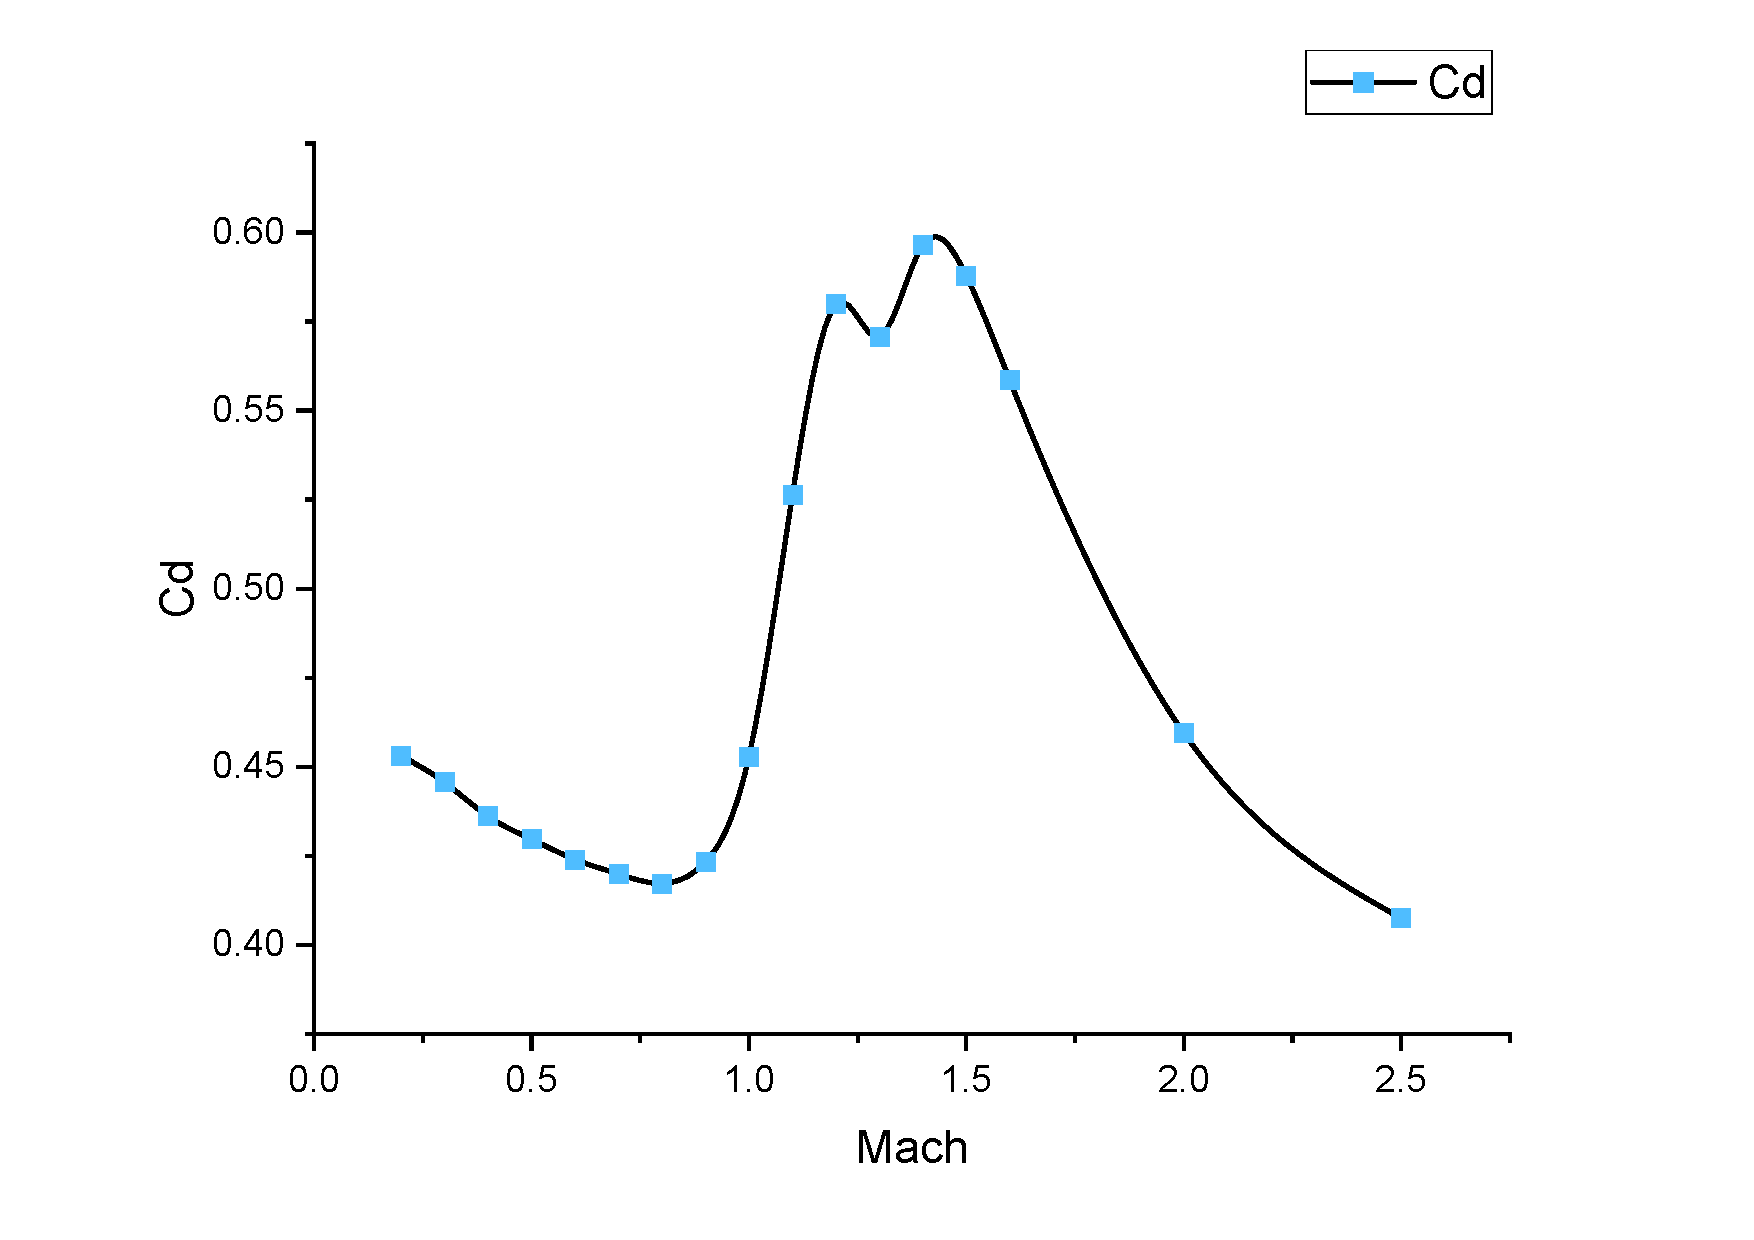
\includegraphics[width=\textwidth]{CD25}
\caption{Graph of drag coefficient for range of 0.2 - 2.5 Mach}
\label{fig:CD25}
\end{figure}

\begin{figure}[H]
\centering
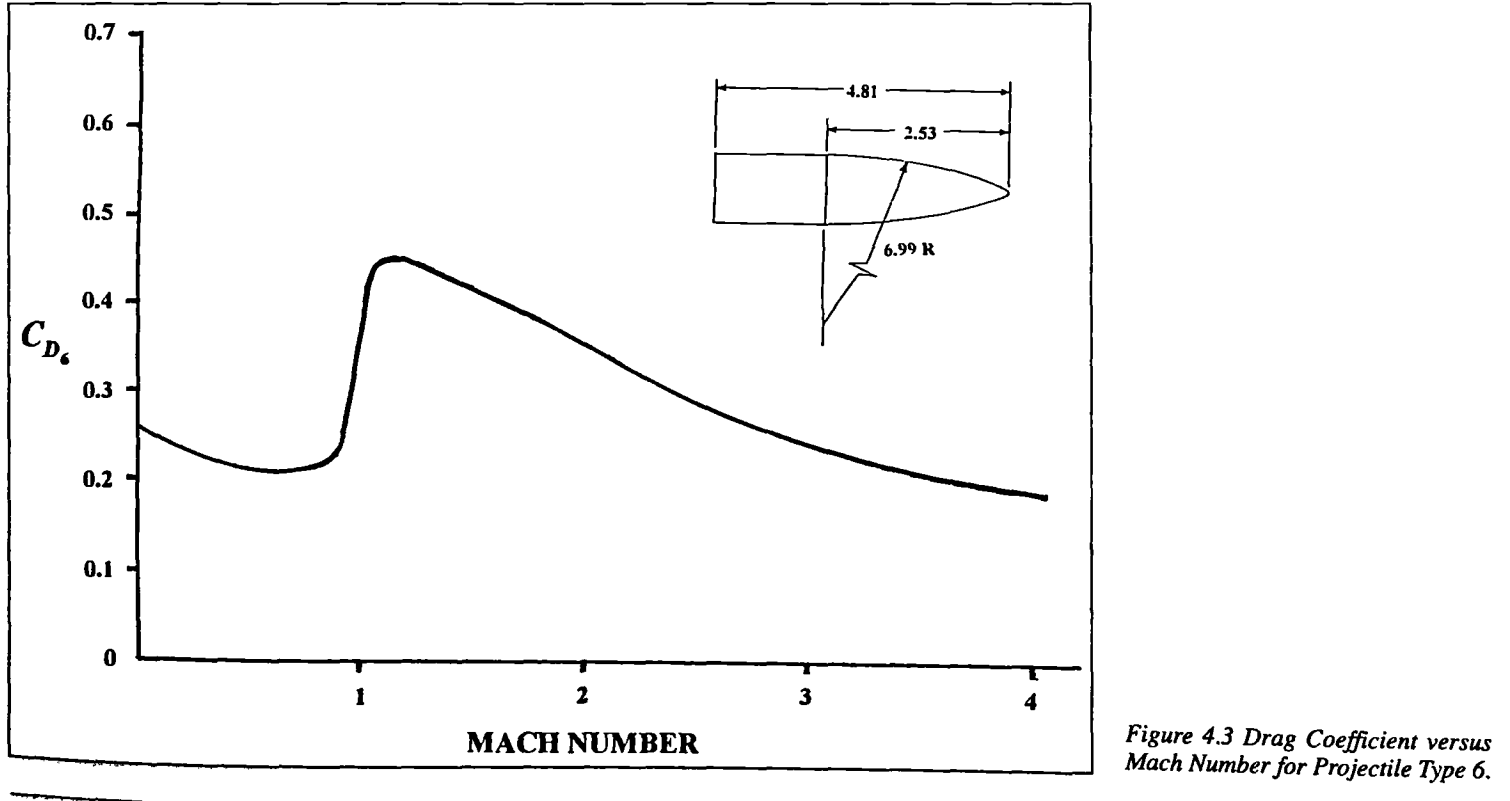
\includegraphics[width=0.8\textwidth]{MEBgraphNOZECONE}
\caption{Graph of drag coefficient for projectal with similar noze cone geometry\cite{MEB}}
\label{fig:MEBgraphNOZECONE}
\end{figure}

\begin{figure}[H]
\centering
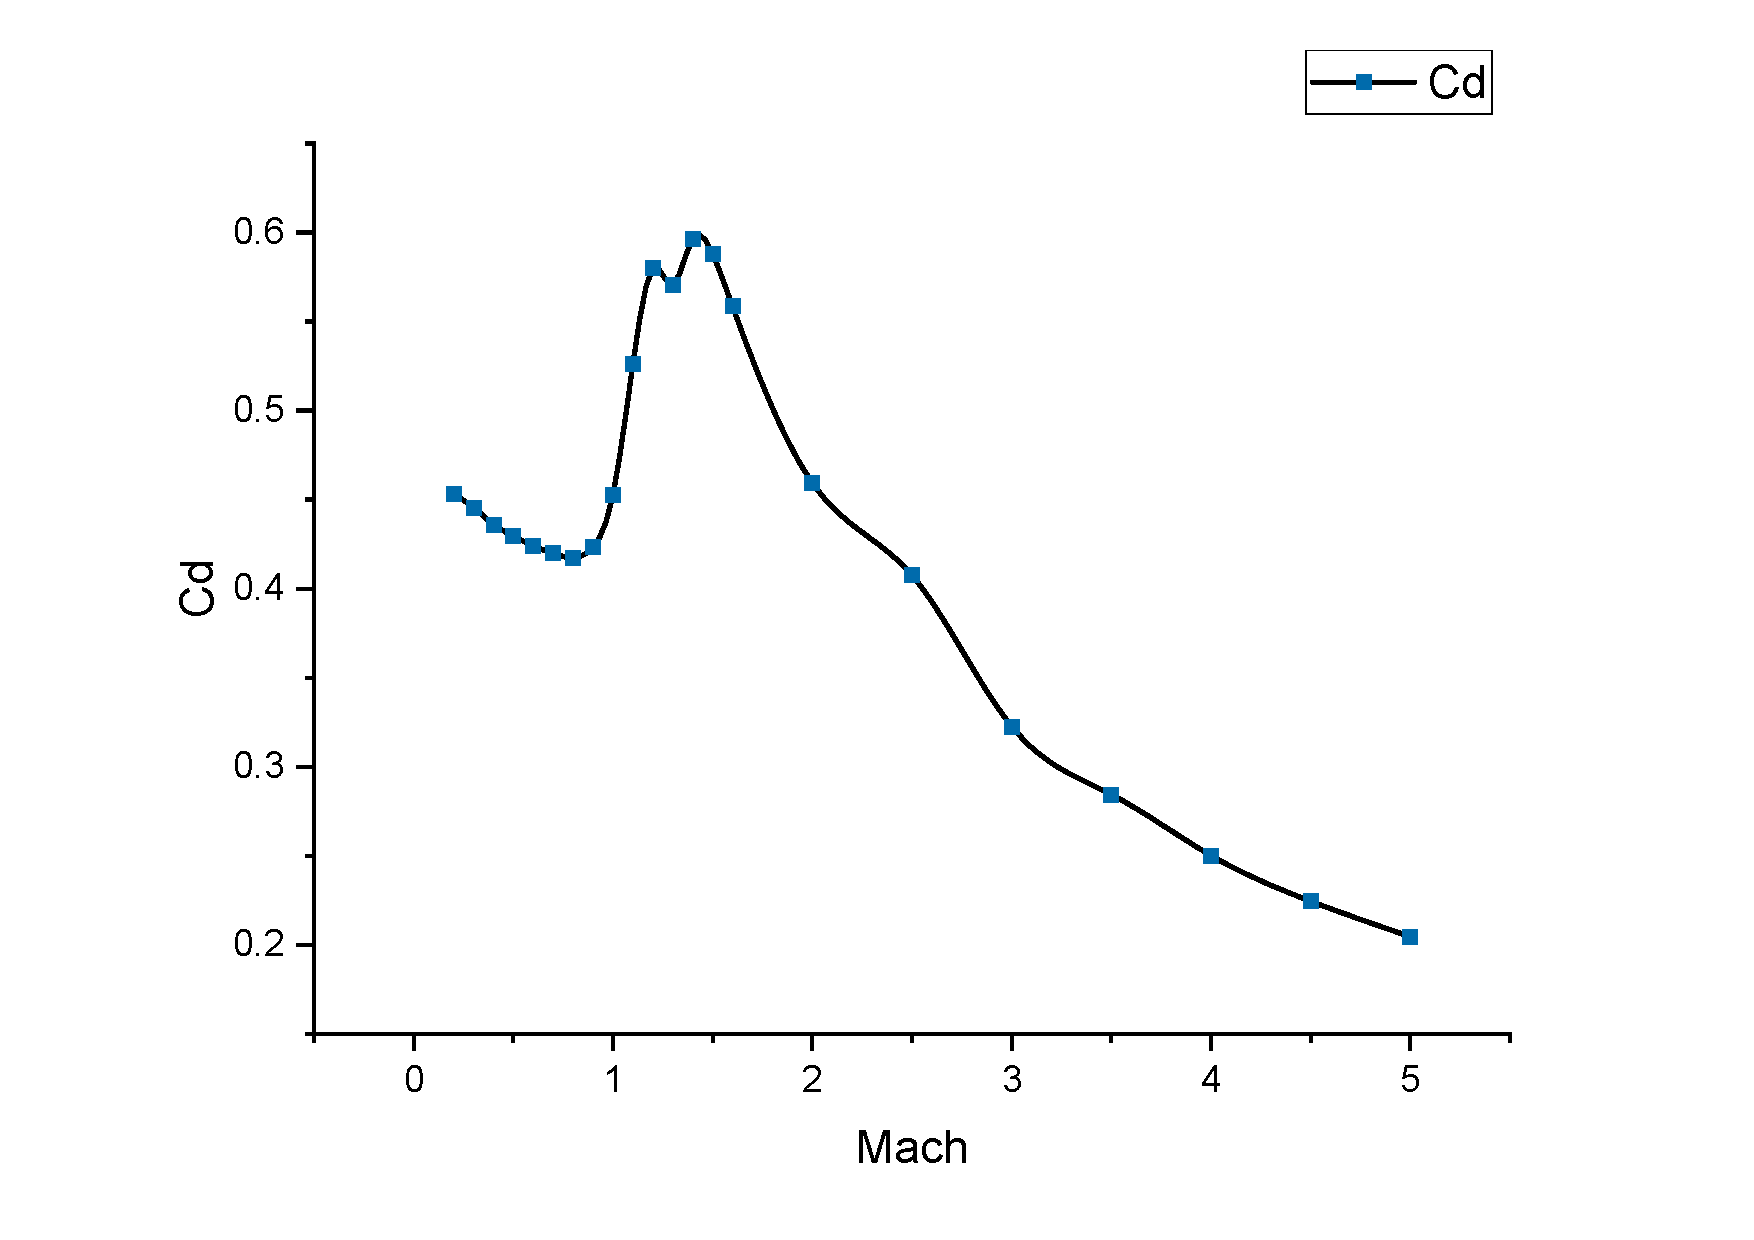
\includegraphics[width=\textwidth]{CD50}
\caption{Graph of drag coefficient for range of 0.2 - 5 Mach}
\label{fig:CD50}
\end{figure}

\begin{figure}[H]
\centering
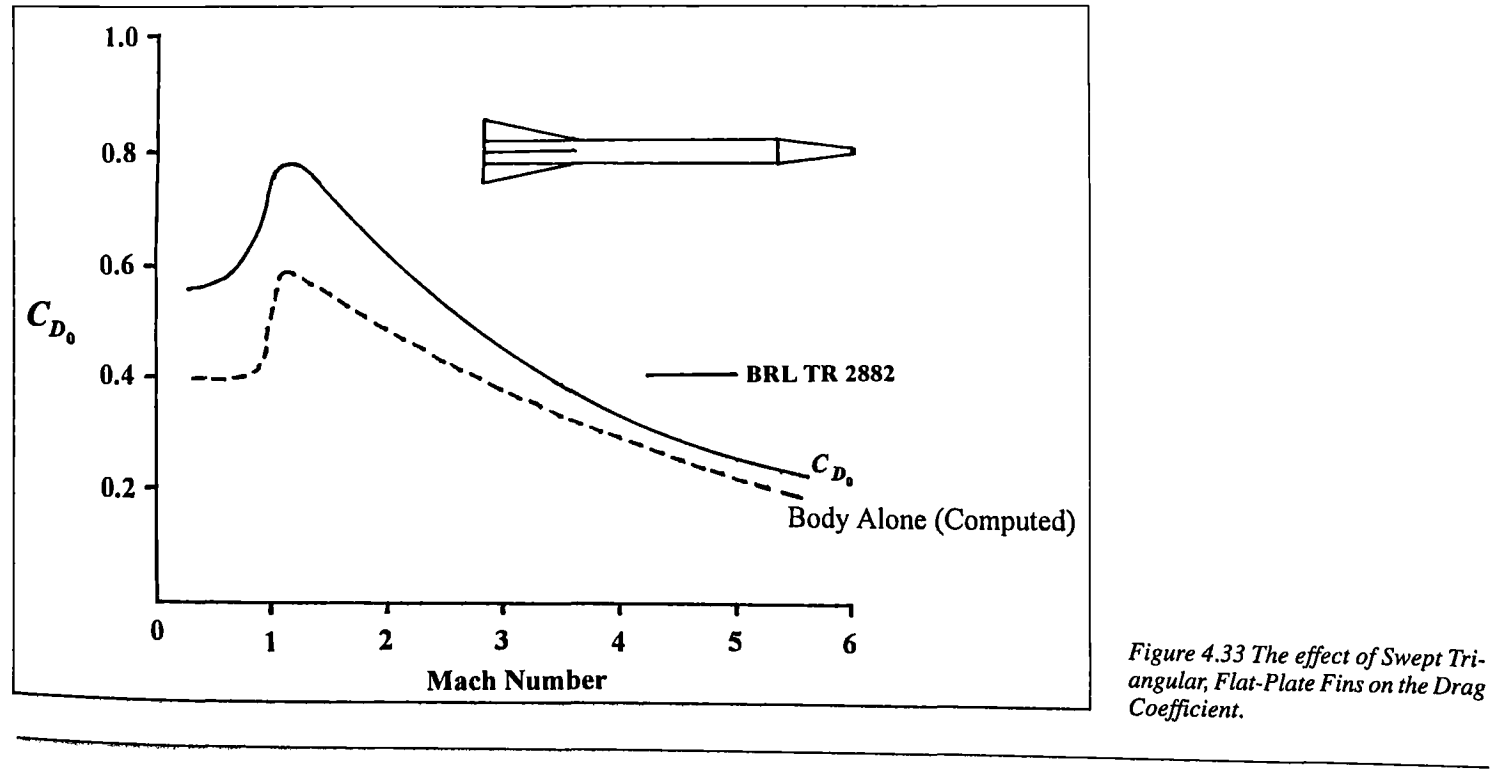
\includegraphics[width=0.8\textwidth]{MEBgraphRocket}
\caption{Graph of drag coefficient for rocket type projectal\cite{MEB}}
\label{fig:MEBgraphRocket}
\end{figure}



\begin{thebibliography}{1}
	\bibitem{MEB}
	Robert L. McCoy (1999) Modern Exterior Ballistics: The Launch and Flight Dynamics of Symmetric Projectiles, Schiffer Military History
\end{thebibliography}

\end{document}